\begin{itemize}
    \item Luego de descargar e instalar Raspberry Pi Imager, se procede a abrir la aplicación y seleccionar el sistema operativo que se desea instalar en la Raspberry Pi. En este caso, se selecciona la opción "Ubuntu".


\begin{figure}[H]
    \centering
    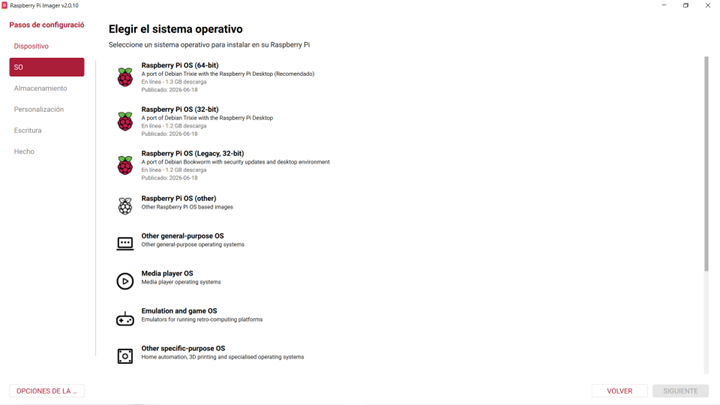
\includegraphics[scale= 0.9]{Pictures/1.png}
    \caption{Elección del sistema operativo en Raspberry Pi Imager}
    \label{CON1}
\end{figure}

\item A continuación, se selecciona la versión de Ubuntu Server 24.04 LTS para arquitectura ARM64, que es compatible con la Raspberry Pi 5.

\begin{figure}[H]
    \centering
    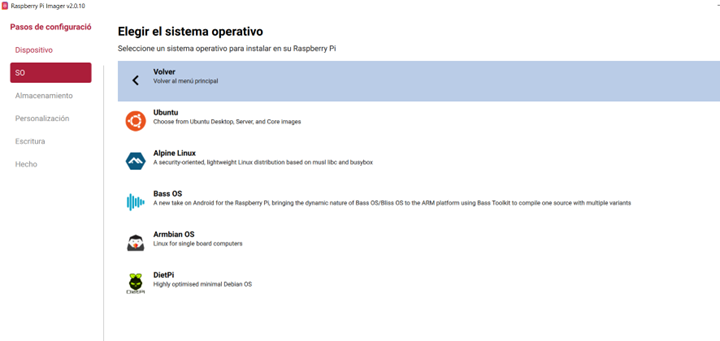
\includegraphics[scale= 0.9]{Pictures/2.png}
    \caption{Selección de la imagen del sistema operativo}
    \label{CON1}
\end{figure}

\begin{figure}[H]
    \centering
    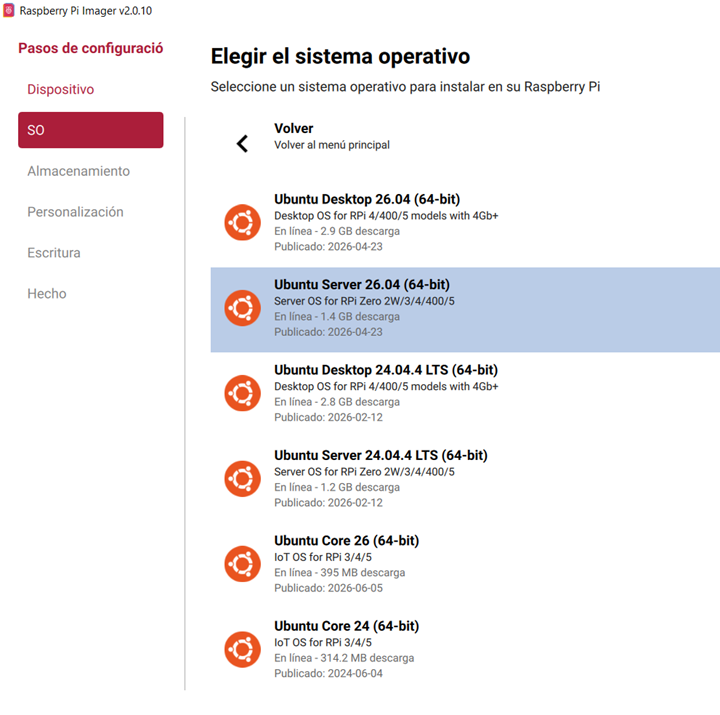
\includegraphics[scale= 0.9]{Pictures/3.png}
    \caption{Confirmación de la selección y versión}
    \label{CON1}
\end{figure}

\item Se debe de colocar un nombre al equipo, asi como el país y la zona horaria correspondiente. Además, se debe de crear un usuario y una contraseña para el acceso al sistema operativo. Por último, se configura la red Wi-Fi a la que se conectará la Raspberry Pi.
\begin{figure}[H]
    \centering
    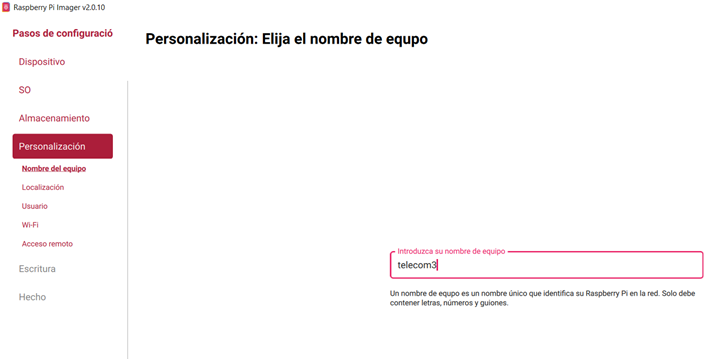
\includegraphics[scale= 0.9]{Pictures/4.png}
    \caption{Elección de nombre de la máquina}
    \label{CON1}
\end{figure}
\begin{figure}[H]
    \centering
    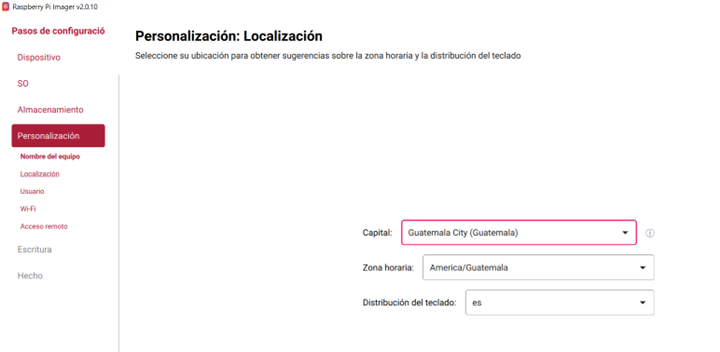
\includegraphics[scale= 0.9]{Pictures/5.png}
    \caption{Selección de país y zona horaria}
    \label{CON1}
\end{figure}

\begin{figure}[H]
    \centering
    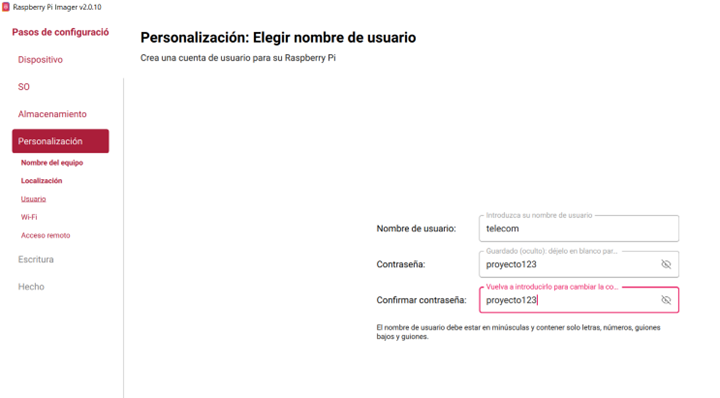
\includegraphics[scale= 0.9]{Pictures/6.png}
    \caption{Configuración de usuario y contraseña}
    \label{CON1}
\end{figure}

\begin{figure}[H]
    \centering
    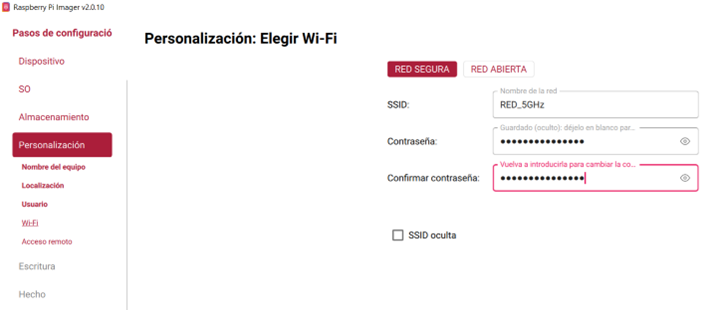
\includegraphics[scale= 0.9]{Pictures/7.png}
    \caption{Configuración de red}
    \label{CON1}
\end{figure}


\item Una vez este todo configurado se procede al resumen de la configuración y a escribir la imagen del sistema operativo en la tarjeta SD. Se debe de tener cuidado de seleccionar la unidad correcta para evitar sobrescribir datos importantes en otras unidades de almacenamiento.
\begin{figure}[H]
    \centering
    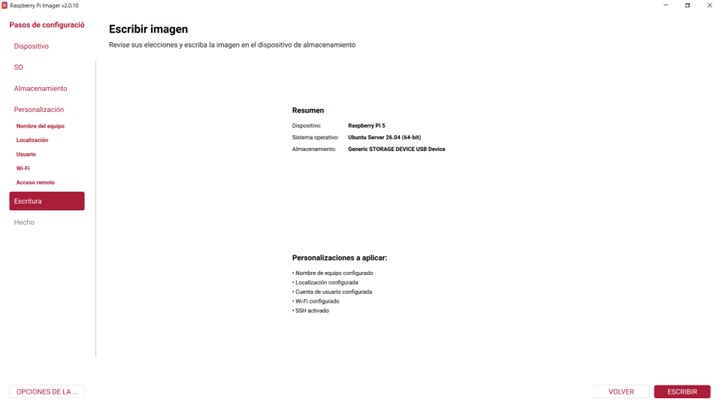
\includegraphics[scale= 0.9]{Pictures/9.png}
    \caption{Confirmación de la configuración y escritura de la imagen en la tarjeta SD}
    \label{CON1}
\end{figure}

\begin{figure}[H]
    \centering
    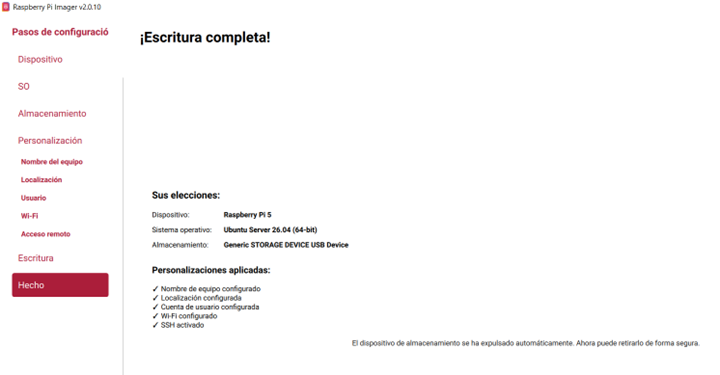
\includegraphics[scale= 0.9]{Pictures/10.png}
    \caption{Finalización del proceso de escritura}
    \label{CON1}
\end{figure}

Luego de estos pasos se inserta el disco SSD en la Raspberry Pi y se procede a encenderla. Se espera a que el sistema operativo se inicie y se realicen las configuraciones iniciales, como la conexión a la red Wi-Fi y la actualización del sistema.

\item Una vez que la Raspberry Pi se encuentra encendida y conectada a la red, se puede acceder a ella de manera remota mediante SSH. Para ello, se utiliza un cliente SSH en otra computadora de la misma red y se ingresa la dirección IP de la Raspberry Pi junto con el nombre de usuario y la contraseña configurados previamente.
\begin{figure}[H]
    \centering
    \includegraphics[scale= 1]{Pictures/CAPTURA.png}
    \caption{Ingreso por SSH a la Raspberry Pi con Ubuntu Server 26.04 LTS}
    \label{CON1}
\end{figure}


\end{itemize}